% !TeX root = LOOK.tex
% Build from a terminal:
% PATH=/Users/mengh/Library/TinyTeX/bin/universal-darwin:$PATH latexmk -pdf LOOK.tex

\documentclass[aspectratio=169,11pt]{beamer}

\usetheme{Madrid}
\usecolortheme{whale}
\usefonttheme{professionalfonts}
\setbeamertemplate{navigation symbols}{}
\setbeamertemplate{blocks}[rounded][shadow=false]

\usepackage[T1]{fontenc}
\usepackage{helvet}
\renewcommand{\familydefault}{\sfdefault}
\usepackage{amsmath,amssymb}
\usepackage{booktabs}
\usepackage{tabularx}
\usepackage{array}
\usepackage{graphicx}
\usepackage{tikz}
\usetikzlibrary{arrows.meta,positioning,calc,fit,backgrounds,decorations.pathreplacing}

\definecolor{LookNavy}{HTML}{17324D}
\definecolor{LookBlue}{HTML}{246B9E}
\definecolor{LookTeal}{HTML}{16827A}
\definecolor{LookOrange}{HTML}{D97706}
\definecolor{LookRed}{HTML}{B42318}
\definecolor{LookInk}{HTML}{172B3A}
\definecolor{LookMuted}{HTML}{5C6B76}
\definecolor{LookLine}{HTML}{D8E1E7}
\definecolor{LookPaleBlue}{HTML}{EAF3F8}
\definecolor{LookPaleTeal}{HTML}{E8F6F3}
\definecolor{LookPaleOrange}{HTML}{FFF3E3}
\definecolor{LookPaper}{HTML}{FAFCFD}

\setbeamercolor{normal text}{fg=LookInk,bg=LookPaper}
\setbeamercolor{structure}{fg=LookBlue}
\setbeamercolor{frametitle}{fg=white,bg=LookNavy}
\setbeamercolor{title}{fg=white}
\setbeamercolor{subtitle}{fg=LookPaleBlue}
\setbeamercolor{block title}{fg=white,bg=LookBlue}
\setbeamercolor{block body}{fg=LookInk,bg=LookPaleBlue}
\setbeamercolor{alertblock title}{fg=white,bg=LookOrange}
\setbeamercolor{alertblock body}{fg=LookInk,bg=LookPaleOrange}
\setbeamercolor{exampleblock title}{fg=white,bg=LookTeal}
\setbeamercolor{exampleblock body}{fg=LookInk,bg=LookPaleTeal}
\setbeamerfont{frametitle}{size=\large,series=\bfseries}
\setbeamerfont{title}{size=\LARGE,series=\bfseries}
\setbeamerfont{subtitle}{size=\large}
\setbeamerfont{block title}{series=\bfseries}
\setbeamersize{text margin left=7mm,text margin right=7mm}

\makeatletter
\setbeamertemplate{footline}{%
  \leavevmode%
  \begin{beamercolorbox}[wd=\paperwidth,ht=2.65ex,dp=1.15ex,leftskip=3mm,rightskip=3mm]{section in head/foot}%
    \usebeamerfont{section in head/foot}%
    \insertsectionnavigationhorizontal{0.82\paperwidth}{}{}%
    \hfill\insertframenumber{} / \inserttotalframenumber
  \end{beamercolorbox}%
}
\makeatother

\setbeamertemplate{itemize item}{\color{LookTeal}\small$\blacktriangleright$}
\setbeamertemplate{itemize subitem}{\color{LookOrange}\scriptsize$\bullet$}

\tikzset{
  flow/.style={-Latex, line width=1.1pt, draw=LookBlue},
  skip/.style={-Latex, line width=1.25pt, draw=LookOrange},
  correction/.style={-Latex, line width=1.4pt, draw=LookTeal},
  stage/.style={rounded corners=2pt, draw=LookLine, fill=white, line width=0.8pt,
                minimum height=8mm, align=center, inner sep=3pt},
  enc/.style={stage, fill=LookPaleBlue, draw=LookBlue},
  dec/.style={stage, fill=LookPaleTeal, draw=LookTeal},
  core/.style={stage, fill=LookPaleOrange, draw=LookOrange},
  note/.style={rounded corners=2pt, draw=LookLine, fill=white, align=left, inner sep=5pt},
}

\newcommand{\takeaway}[1]{%
  \vfill
  \begin{beamercolorbox}[rounded=true,sep=0.7ex,leftskip=0.8ex]{block body}%
    \textbf{Take-home:} #1
  \end{beamercolorbox}%
}
\newcommand{\statuspill}[2]{%
  \tikz[baseline=-0.55ex]\node[rounded corners=2pt,fill=#1,inner xsep=5pt,inner ysep=2.2pt]
  {\scriptsize\bfseries #2};%
}
\newcolumntype{Y}{>{\raggedright\arraybackslash}X}
\newcolumntype{C}{>{\centering\arraybackslash}X}

\title[LOOK in MHD V4]{LOOK in MHD Framework V4}
\subtitle{Plug-and-play linear latent correction for missing-modality segmentation}
\author[Meng Haoding]{Meng Haoding}
\institute{PhD Supervisor Discussion}
\date{August 2026}

\begin{document}

% -----------------------------------------------------------------------------
\begin{frame}[plain]
  \begin{tikzpicture}[remember picture,overlay]
    \fill[LookNavy] (current page.south west) rectangle (current page.north east);
    \fill[LookTeal] (current page.south west) rectangle ([xshift=2.8mm]current page.north west);
    \node[anchor=north west,text width=11.7cm,align=left] at
      ([xshift=11mm,yshift=-14mm]current page.north west) {\usebeamerfont{title}\color{white}\inserttitle};
    \node[anchor=north west,text width=11.7cm,align=left] at
      ([xshift=11mm,yshift=-29mm]current page.north west) {\usebeamerfont{subtitle}\color{LookPaleBlue}\insertsubtitle};
    \node[anchor=north west,rounded corners=2pt,fill=LookTeal,text=white,
          inner xsep=7pt,inner ysep=4pt] at
      ([xshift=11mm,yshift=-47mm]current page.north west) {\small PhD foundation: MHD V4};
    \node[anchor=north west,rounded corners=2pt,fill=LookOrange,text=white,
          inner xsep=7pt,inner ysep=4pt] at
      ([xshift=58mm,yshift=-47mm]current page.north west) {\small First side work: LOOK};
    \draw[white!35,line width=0.8pt] ([xshift=11mm,yshift=17mm]current page.south west)
      -- ([xshift=-11mm,yshift=17mm]current page.south east);
    \node[anchor=south west,text=white!85] at ([xshift=11mm,yshift=7mm]current page.south west)
      {\small \insertauthor\quad|\quad\insertinstitute};
    \node[anchor=south east,text=white!65] at ([xshift=-11mm,yshift=7mm]current page.south east)
      {\small \insertdate};
  \end{tikzpicture}
\end{frame}

% -----------------------------------------------------------------------------
\begin{frame}{Storyline for this discussion}
  \tableofcontents
  \vspace{1mm}
  \begin{exampleblock}{One sentence}
    MHD V4 exposes the internal computation graph; LOOK uses that access to estimate and inject a
    lightweight linear correction when MRI modalities are missing.
  \end{exampleblock}
\end{frame}

% =============================================================================
\section{Motivation}

\begin{frame}{Clinical problem: multimodal MRI is informative, but often incomplete}
  \begin{columns}[T,onlytextwidth]
    \column{0.57\textwidth}
      \begin{itemize}
        \item Complementary MRI contrasts encode different tissue and lesion characteristics.
        \item In practice, a sequence can be unavailable, corrupted, or omitted because of time,
              motion, protocol, or scanner constraints.
        \item A segmentation model trained for complete inputs can then receive an out-of-distribution
              input and lose clinically relevant information.
      \end{itemize}
    \column{0.41\textwidth}
      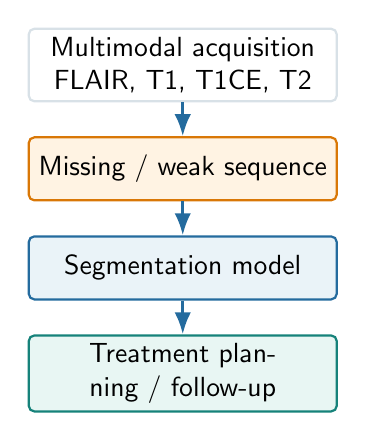
\begin{tikzpicture}[node distance=4.3mm]
        \node[stage,text width=3.7cm] (a) {Multimodal acquisition\\FLAIR, T1, T1CE, T2};
        \node[core,text width=3.7cm,below=of a] (b) {Missing / weak sequence};
        \node[enc,text width=3.7cm,below=of b] (c) {Segmentation model};
        \node[dec,text width=3.7cm,below=of c] (d) {Treatment planning / follow-up};
        \draw[flow] (a) -- (b);
        \draw[flow] (b) -- (c);
        \draw[flow] (c) -- (d);
      \end{tikzpicture}
  \end{columns}
  \takeaway{The robustness problem begins at the input, but its consequences appear at the clinical endpoint.}
\end{frame}

\begin{frame}{Where LOOK sits in the medical image processing pipeline}
  \centering
  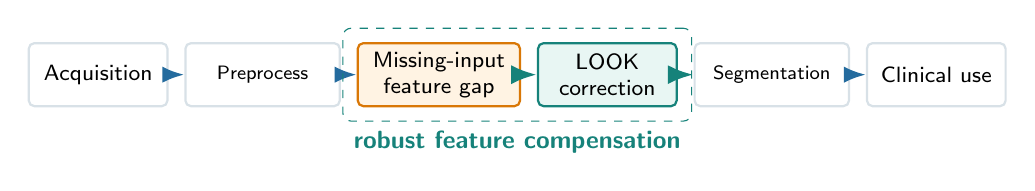
\begin{tikzpicture}[node distance=2mm,font=\footnotesize,
      every node/.append style={inner xsep=2pt}]
    \node[stage,text width=1.55cm] (raw) {Acquisition};
    \node[stage,text width=1.75cm,right=of raw,font=\scriptsize] (prep) {Preprocess};
    \node[core,text width=1.85cm,right=of prep] (miss) {Missing-input\\feature gap};
    \node[dec,text width=1.55cm,right=of miss] (look) {LOOK\\correction};
    \node[stage,text width=1.75cm,right=of look,font=\scriptsize] (seg) {Segmentation};
    \node[stage,text width=1.55cm,right=of seg] (clinical) {Clinical use};
    \draw[flow] (raw) -- (prep);
    \draw[flow] (prep) -- (miss);
    \draw[correction] (miss) -- (look);
    \draw[correction] (look) -- (seg);
    \draw[flow] (seg) -- (clinical);
    \node[draw=LookTeal,dashed,rounded corners=3pt,fit=(miss)(look),inner sep=5pt,
          label={[text=LookTeal,font=\bfseries\small]below:robust feature compensation}] {};
  \end{tikzpicture}
  \vspace{7mm}
  \begin{block}{Research positioning}
    LOOK is not a new segmentation backbone and not a pseudo-image generator. It estimates the
    missing-to-full feature discrepancy at an accessible network state and writes back a residual.
  \end{block}
\end{frame}

% =============================================================================
\section{MHD V4}

\begin{frame}{Why MHD Framework is the PhD foundation}
  \begin{columns}[T,onlytextwidth]
    \column{0.48\textwidth}
      \begin{alertblock}{Conventional view}
        A model is called as a monolithic forward function. Intermediate states are temporary and
        interventions require model-specific hooks or rewrites.
      \end{alertblock}
    \column{0.48\textwidth}
      \begin{exampleblock}{MHD view}
        A model is represented as named nodes, executable hyperedges, and level-wise topology.
        Intermediate states become explicit intervention points.
      \end{exampleblock}
  \end{columns}
  \vspace{3mm}
  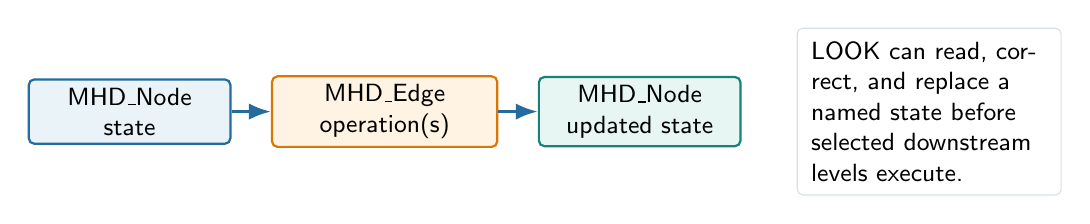
\begin{tikzpicture}[node distance=5mm,font=\small]
    \node[enc,text width=2.35cm] (n1) {MHD\_Node\\state};
    \node[core,text width=2.65cm,right=of n1] (e) {MHD\_Edge\\operation(s)};
    \node[dec,text width=2.35cm,right=of e] (n2) {MHD\_Node\\updated state};
    \draw[flow] (n1) -- (e);
    \draw[flow] (e) -- (n2);
    \node[note,text width=3.0cm,right=7mm of n2] {LOOK can read, correct, and replace a named state
      before selected downstream levels execute.};
  \end{tikzpicture}
\end{frame}

\begin{frame}{MHD V4: code-level contract used by LOOK}
  \small
  \begin{tabularx}{\textwidth}{>{\bfseries\color{LookNavy}}p{2.35cm} Y Y}
    \toprule
    Component & Implemented behavior & Why it matters for LOOK \\
    \midrule
    MHD\_Node & \texttt{initial\_state} and \texttt{current\_state}; replace/add/concat transfer modes
      & A stable state can be reset, observed, and overwritten with a correction. \\
    MHD\_Edge & Executes an \texttt{nn.Module}, tensor-op string, callable, or partial
      & Existing network operations remain reusable inside the graph. \\
    MHD\_Topo & Per-level role matrices and sort matrices encode incidence and input/output order
      & Multi-input decoder blocks preserve ordered skip features. \\
    MHD\_Graph & \texttt{forward(levels=[...])} runs selected execution levels
      & Run to a node, inject LOOK, then continue downstream. \\
    \bottomrule
  \end{tabularx}
  \vspace{2mm}
  \begin{exampleblock}{Current graph instance}
    14 nodes, 12 hyperedges, and 12 execution levels, including logits, loss, and Dice states.
  \end{exampleblock}
\end{frame}

\begin{frame}{Current backbone: the actual 3D U-Net graph includes four skip connections}
  \centering
  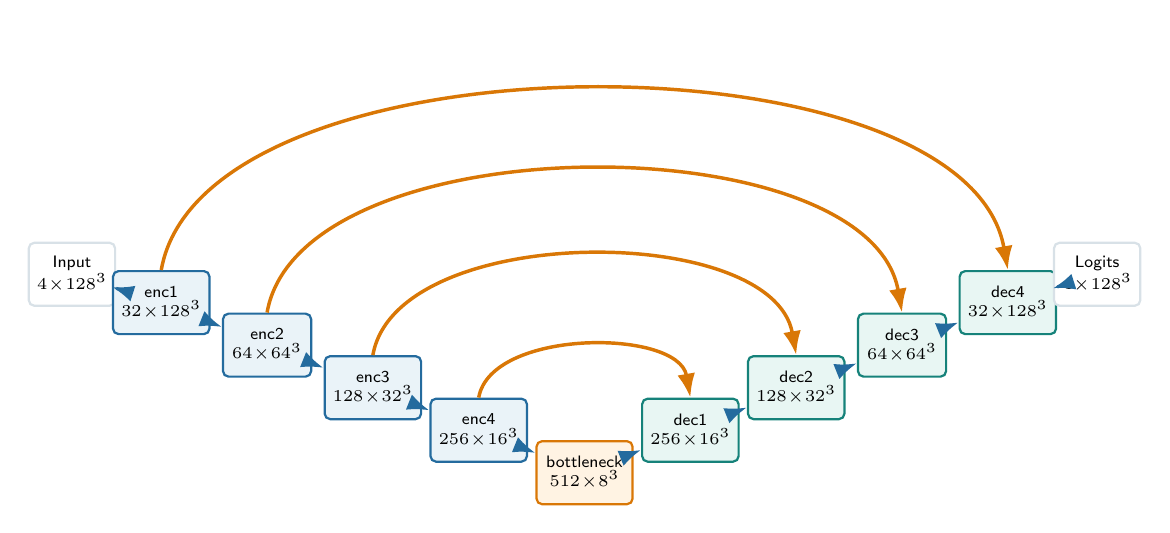
\begin{tikzpicture}[x=0.84cm,y=0.72cm,font=\fontsize{6.1}{6.9}\selectfont]
    \node[stage,minimum width=1.05cm] (in) at (0,4.1) {Input\\$4\!\times\!128^3$};
    \node[enc,minimum width=1.12cm] (e1) at (1.35,3.6) {enc1\\$32\!\times\!128^3$};
    \node[enc,minimum width=1.12cm] (e2) at (2.95,2.85) {enc2\\$64\!\times\!64^3$};
    \node[enc,minimum width=1.12cm] (e3) at (4.55,2.10) {enc3\\$128\!\times\!32^3$};
    \node[enc,minimum width=1.12cm] (e4) at (6.15,1.35) {enc4\\$256\!\times\!16^3$};
    \node[core,minimum width=1.22cm] (b) at (7.75,0.60) {bottleneck\\$512\!\times\!8^3$};
    \node[dec,minimum width=1.12cm] (d1) at (9.35,1.35) {dec1\\$256\!\times\!16^3$};
    \node[dec,minimum width=1.12cm] (d2) at (10.95,2.10) {dec2\\$128\!\times\!32^3$};
    \node[dec,minimum width=1.12cm] (d3) at (12.55,2.85) {dec3\\$64\!\times\!64^3$};
    \node[dec,minimum width=1.12cm] (d4) at (14.15,3.60) {dec4\\$32\!\times\!128^3$};
    \node[stage,minimum width=1.05cm] (out) at (15.5,4.1) {Logits\\$4\!\times\!128^3$};
    \draw[flow] (in) -- (e1);
    \draw[flow] (e1) -- (e2);
    \draw[flow] (e2) -- (e3);
    \draw[flow] (e3) -- (e4);
    \draw[flow] (e4) -- (b);
    \draw[flow] (b) -- (d1);
    \draw[flow] (d1) -- (d2);
    \draw[flow] (d2) -- (d3);
    \draw[flow] (d3) -- (d4);
    \draw[flow] (d4) -- (out);
    \draw[skip] (e4.north) to[out=80,in=100,looseness=0.85] (d1.north);
    \draw[skip] (e3.north) to[out=80,in=100,looseness=0.82] (d2.north);
    \draw[skip] (e2.north) to[out=80,in=100,looseness=0.78] (d3.north);
    \draw[skip] (e1.north) to[out=80,in=100,looseness=0.74] (d4.north);
  \end{tikzpicture}
  \takeaway{The skip tensors are explicit second inputs to the four \texttt{UpConcat} hyperedges.}
\end{frame}

% =============================================================================
\section{LOOK}

\begin{frame}{Problem setting in the current notebook demo}
  \begin{columns}[T,onlytextwidth]
    \column{0.48\textwidth}
      \begin{block}{Reference path}
        \centering
        Full input: FLAIR + T1 + T1CE + T2\\[2mm]
        Feature at node $\ell$: $x^{(\ell)}_{\mathrm{full}}$
      \end{block}
    \column{0.48\textwidth}
      \begin{alertblock}{Missing path}
        \centering
        Current pattern: FLAIR, T1, T2 removed\\[2mm]
        Only T1CE is retained: $x^{(\ell)}_{\mathrm{miss}}$
      \end{alertblock}
  \end{columns}
  \vspace{3mm}
  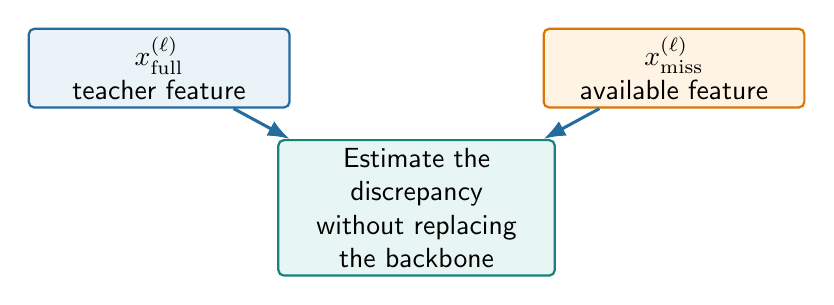
\begin{tikzpicture}[node distance=8mm]
    \node[enc,text width=3.1cm] (full) {$x^{(\ell)}_{\mathrm{full}}$\\teacher feature};
    \node[core,text width=3.1cm,right=32mm of full] (miss) {$x^{(\ell)}_{\mathrm{miss}}$\\available feature};
    \node[dec,text width=3.3cm,below=9mm of $(full)!0.5!(miss)$] (goal)
      {Estimate the discrepancy\\without replacing the backbone};
    \draw[flow] (full) -- (goal);
    \draw[flow] (miss) -- (goal);
  \end{tikzpicture}
  \takeaway{The present feasibility experiment studies one severe missing pattern; the method definition is broader.}
\end{frame}

\begin{frame}{LOOK: a linear residual map in a compact latent space}
  \begin{columns}[T,onlytextwidth]
    \column{0.54\textwidth}
      \begin{align*}
        z_{\mathrm{miss}} &= P\!\left(\mathcal{N}(D(x_{\mathrm{miss}}))\right),\\
        \Delta z &= z_{\mathrm{miss}}W+b,\\
        \widehat{x}_{\mathrm{corr}} &= x_{\mathrm{miss}}
          + \alpha\,U\!\left(P^{\top}\Delta z\right).
      \end{align*}
      \footnotesize
      $D/U$: spatial down/up-sampling; $\mathcal{N}$: stored feature normalization;
      $P$: PCA projection; $W,b$: ridge correction; $\alpha$: node-wise injection strength.
    \column{0.43\textwidth}
      \begin{exampleblock}{What is linear?}
        PCA encoding/decoding and the learned correction $zW+b$ are linear or affine. LOOK adds no
        nonlinear generator or new nonlinear segmentation module.
      \end{exampleblock}
      \begin{alertblock}{Precise claim}
        LOOK itself does not require nonlinear backbone retraining. The current notebook applies it
        to an already fine-tuned missing-pattern backbone.
      \end{alertblock}
  \end{columns}
\end{frame}

\begin{frame}{How the correction is estimated}
  \centering
  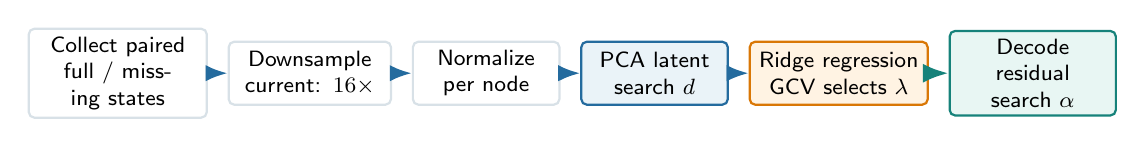
\begin{tikzpicture}[node distance=2.5mm,font=\footnotesize]
    \node[stage,text width=2.05cm] (collect) {Collect paired\\full / missing states};
    \node[stage,text width=1.85cm,right=of collect] (down) {Downsample\\current: $16\times$};
    \node[stage,text width=1.65cm,right=of down] (norm) {Normalize\\per node};
    \node[enc,text width=1.65cm,right=of norm] (pca) {PCA latent\\search $d$};
    \node[core,text width=2.05cm,right=of pca] (ridge) {Ridge regression\\GCV selects $\lambda$};
    \node[dec,text width=1.9cm,right=of ridge] (inject) {Decode residual\\search $\alpha$};
    \draw[flow] (collect) -- (down);
    \draw[flow] (down) -- (norm);
    \draw[flow] (norm) -- (pca);
    \draw[flow] (pca) -- (ridge);
    \draw[correction] (ridge) -- (inject);
  \end{tikzpicture}
  \vspace{5mm}
  \begin{block}{Closed-form correction}
    With centered latent pairs, ridge solves
    $W=(Z_m^{\top}Z_m+\lambda I)^{-1}Z_m^{\top}(Z_f-Z_m)$;
    the intercept $b$ restores the means, and GCV selects $\lambda$.
  \end{block}
  \takeaway{The expensive backbone is reused; fitting LOOK is a small paired linear estimation problem at each node.}
\end{frame}

\begin{frame}{MHD level-wise execution makes injection explicit}
  \centering
  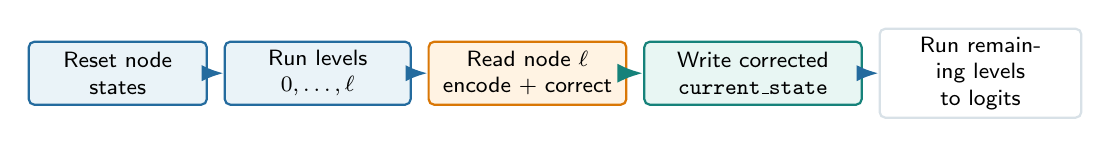
\begin{tikzpicture}[node distance=2mm,font=\footnotesize]
    \node[enc,text width=2.05cm] (reset) {Reset node states};
    \node[enc,text width=2.15cm,right=of reset] (run) {Run levels\\$0,\ldots,\ell$};
    \node[core,text width=2.3cm,right=of run] (read) {Read node $\ell$\\encode + correct};
    \node[dec,text width=2.55cm,right=of read] (write) {Write corrected\\\texttt{current\_state}};
    \node[stage,text width=2.35cm,right=of write] (continue) {Run remaining levels\\to logits};
    \draw[flow] (reset) -- (run);
    \draw[flow] (run) -- (read);
    \draw[correction] (read) -- (write);
    \draw[flow] (write) -- (continue);
  \end{tikzpicture}
  \vspace{5mm}
  \begin{columns}[T,onlytextwidth]
    \column{0.48\textwidth}
      \begin{exampleblock}{Candidate nodes}
        input, enc1--enc4, bottleneck, dec1--dec4
      \end{exampleblock}
    \column{0.48\textwidth}
      \begin{block}{Key abstraction}
        LOOK depends on an accessible state and an execution boundary, not on a hard-coded U-Net class.
      \end{block}
  \end{columns}
\end{frame}

\begin{frame}{Why LOOK is designed to transfer}
  \begin{columns}[T,onlytextwidth]
    \column{0.32\textwidth}
      \begin{exampleblock}{Plug-and-play}
        Fit and inject a small correction while keeping the nonlinear backbone fixed.
      \end{exampleblock}
    \column{0.32\textwidth}
      \begin{exampleblock}{Composable}
        Apply after zero/mean filling, synthesis, modality dropout, or fine-tuning.
      \end{exampleblock}
    \column{0.32\textwidth}
      \begin{exampleblock}{Inspectable}
        Analyze $W$, singular values, eigen-structure, rank, and node stability.
      \end{exampleblock}
  \end{columns}
  \vspace{5mm}
  \begin{alertblock}{Boundary of the claim}
    Transferability is a design hypothesis supported by a working demo. It still requires controlled
    experiments across missing patterns, datasets, backbones, and acquisition domains.
  \end{alertblock}
\end{frame}

% =============================================================================
\section{Evidence}

\begin{frame}{Current demo configuration: what has actually been run}
  \small
  \begin{tabularx}{\textwidth}{>{\bfseries\color{LookNavy}}p{3.0cm} Y}
    \toprule
    Item & Notebook configuration \\
    \midrule
    Data & BraTS 2020 training cases re-split 70/15/15: 258 train, 55 validation, 56 test \\
    Input / task & $128^3$, four MRI channels, four-class voxel prediction; Dice reported for NCR, ED, ET \\
    Backbone & MHD-mapped 3D U-Net; base channels 32; SGD + polynomial LR + early stopping \\
    Missing pattern & \texttt{missing\_FLAIR\_T1\_T2}: only T1CE retained \\
    LOOK nodes & input, enc1--enc4, bottleneck, and dec1--dec4 \\
    Compression & Current spatial downsampling factor 16; PCA dimension and ridge $\lambda$ searched \\
    Status & End-to-end pipeline executed; validation improvement observed \\
    \bottomrule
  \end{tabularx}
\end{frame}

\begin{frame}{Preliminary validation: a positive signal, not a final claim}
  \begin{columns}[T,onlytextwidth]
    \column{0.57\textwidth}
      \begin{table}
        \footnotesize
        \setlength{\tabcolsep}{3pt}
        \begin{tabular}{lrrrr}
          \toprule
          Configuration & Mean & NCR & ED & ET \\
          \midrule
          Missing baseline & 0.6332 & 0.6213 & 0.5312 & 0.7471 \\
          LOOK, output A & \textbf{0.6413} & 0.6249 & 0.5185 & \textbf{0.7803} \\
          LOOK, output B & 0.6370 & 0.6246 & 0.5147 & 0.7717 \\
          \bottomrule
        \end{tabular}
      \end{table}
      \footnotesize Validation set only; one severe missing pattern. Output A gives
      $\Delta$Mean Dice $=+0.0081$; output B gives $+0.0038$.
    \column{0.40\textwidth}
      \resizebox{\linewidth}{!}{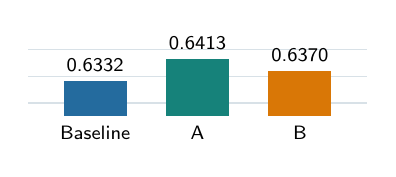
\begin{tikzpicture}[x=1cm,y=34cm,font=\scriptsize]
        \draw[LookLine] (0,0.625) -- (4.3,0.625);
        \draw[LookLine] (0,0.635) -- (4.3,0.635);
        \draw[LookLine] (0,0.645) -- (4.3,0.645);
        \fill[LookBlue] (0.45,0.620) rectangle (1.25,0.6332);
        \fill[LookTeal] (1.75,0.620) rectangle (2.55,0.6413);
        \fill[LookOrange] (3.05,0.620) rectangle (3.85,0.6370);
        \node[below] at (0.85,0.620) {Baseline};
        \node[below] at (2.15,0.620) {A};
        \node[below] at (3.45,0.620) {B};
        \node[above] at (0.85,0.6332) {0.6332};
        \node[above] at (2.15,0.6413) {0.6413};
        \node[above] at (3.45,0.6370) {0.6370};
      \end{tikzpicture}}
  \end{columns}
  \begin{alertblock}{Required next step}
    The two stored notebook outputs differ, and ED decreases while ET improves. Freeze the exact
    correction state, seed, and alpha dictionary, then rerun validation and untouched test evaluation.
  \end{alertblock}
\end{frame}

\begin{frame}{What the current evidence does and does not establish}
  \begin{columns}[T,onlytextwidth]
    \column{0.48\textwidth}
      \begin{exampleblock}{Supported now}
        \begin{itemize}
          \item The full pipeline runs end-to-end.
          \item A linear latent residual can improve validation Mean Dice.
          \item Decoder-side correction can recover ET signal in this setting.
          \item MHD provides usable intervention points.
        \end{itemize}
      \end{exampleblock}
    \column{0.48\textwidth}
      \begin{alertblock}{Not established yet}
        \begin{itemize}
          \item Statistical significance or confidence intervals
          \item Generalization to other missing patterns
          \item Benefit on an untouched test set
          \item Superiority over synthesis or robust-training baselines
          \item Cross-center or cross-backbone transfer
        \end{itemize}
      \end{alertblock}
  \end{columns}
\end{frame}

\begin{frame}{Comparison landscape: LOOK is a correction layer, not a closed pipeline}
  \centering
  \resizebox{0.97\textwidth}{!}{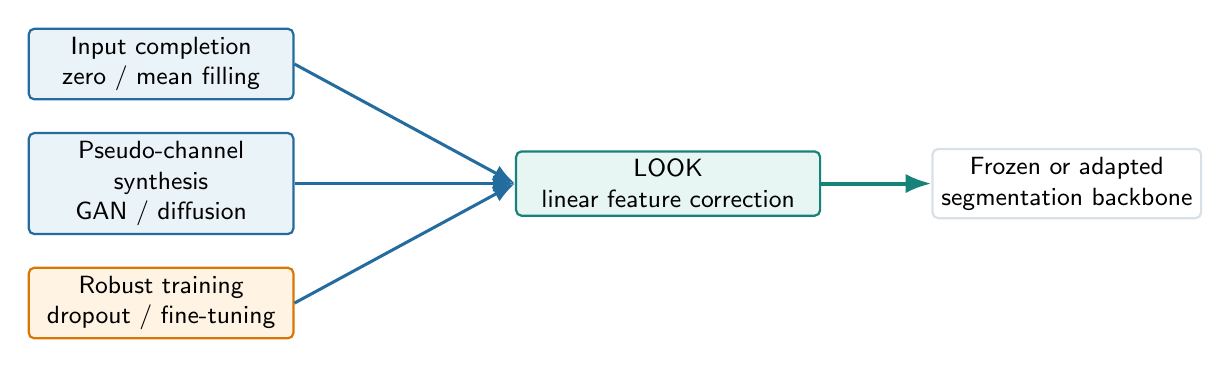
\begin{tikzpicture}[node distance=4mm,font=\small]
    \node[enc,text width=3.15cm] (fill) {Input completion\\zero / mean filling};
    \node[enc,text width=3.15cm,below=of fill] (synth) {Pseudo-channel synthesis\\GAN / diffusion};
    \node[core,text width=3.15cm,below=of synth] (train) {Robust training\\dropout / fine-tuning};
    \node[dec,text width=3.65cm,right=28mm of synth] (look) {LOOK\\linear feature correction};
    \node[stage,text width=3.2cm,right=14mm of look] (seg) {Frozen or adapted\\segmentation backbone};
    \draw[flow] (fill.east) -- (look.west);
    \draw[flow] (synth.east) -- (look.west);
    \draw[flow] (train.east) -- (look.west);
    \draw[correction] (look) -- (seg);
  \end{tikzpicture}}
  \vspace{2mm}
  \begin{block}{Evaluation logic}
    Compare each baseline alone and with LOOK added afterward. This separates the value of input
    recovery or nonlinear adaptation from the incremental value of linear feature correction.
  \end{block}
\end{frame}

% =============================================================================
\section{Expansion}

\begin{frame}{A decision-complete experiment matrix}
  \scriptsize
  \begin{tabularx}{\textwidth}{>{\bfseries\color{LookNavy}}p{2.4cm} Y Y Y}
    \toprule
    Axis & Minimum study & Extended study & Primary readout \\
    \midrule
    Missingness & Every single missing modality & Double/triple and clinically non-random patterns
      & Mean + class Dice; worst-case robustness \\
    Downsampling & $2\times,4\times,8\times,16\times$ & $1\times$ where memory permits
      & Accuracy, memory, fit time, inference overhead \\
    Injection node & Each input, encoder, bottleneck, and decoder node & Greedy and joint multi-node sets
      & Incremental gain and node stability \\
    Baseline & zero, mean, modality dropout, missing-input fine-tune & GAN/diffusion and joint fine-tune
      & Baseline vs baseline+LOOK \\
    Backbone & Current 3D U-Net & 2D, 2.5D, large/foundation segmentation models
      & Transfer without nonlinear retraining \\
    Domain & BraTS internal split & Multicenter cardiac MRI, scanner/protocol shifts
      & Cross-center generalization and calibration \\
    \bottomrule
  \end{tabularx}
  \takeaway{The paper should test a method property, not optimize a single favorable configuration.}
\end{frame}

\begin{frame}{Interpreting the correction matrix can become a scientific contribution}
  \begin{columns}[T,onlytextwidth]
    \column{0.50\textwidth}
      \begin{itemize}
        \item Singular-value spectrum and effective rank of $W$
        \item Eigenvalue and eigenvector analysis for an appropriate square or symmetric operator
        \item Layer-wise stability across seeds, folds, centers, and missing patterns
        \item Principal directions associated with ET, ED, and NCR recovery
        \item Alignment between correction directions and full-to-missing feature shift
      \end{itemize}
    \column{0.47\textwidth}
      \resizebox{0.96\linewidth}{!}{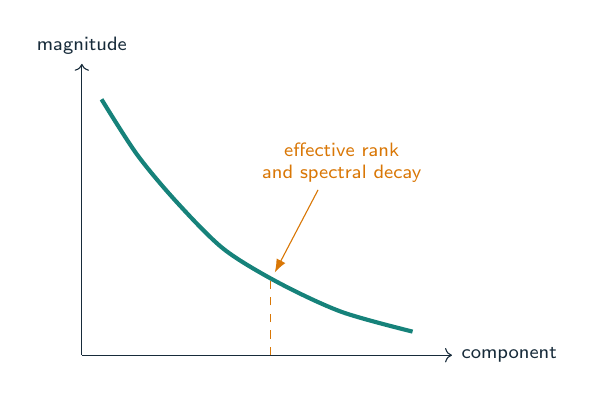
\begin{tikzpicture}[font=\scriptsize]
        \draw[->,LookInk] (0,0) -- (4.7,0) node[right] {component};
        \draw[->,LookInk] (0,0) -- (0,3.7) node[above] {magnitude};
        \draw[LookTeal,line width=1.5pt] plot[smooth] coordinates
          {(0.25,3.25) (0.7,2.55) (1.2,1.95) (1.8,1.35) (2.5,0.92) (3.3,0.55) (4.2,0.30)};
        \draw[LookOrange,dashed] (2.4,0) -- (2.4,1.0);
        \node[align=center,text=LookOrange] at (3.3,2.45) {effective rank\\and spectral decay};
        \draw[-Latex,LookOrange] (3.0,2.1) -- (2.45,1.05);
      \end{tikzpicture}}
      \begin{exampleblock}{Interpretability question}
        Which low-dimensional directions consistently encode the information lost with a modality?
      \end{exampleblock}
  \end{columns}
\end{frame}

\begin{frame}{Roadmap: data, models, and system scale}
  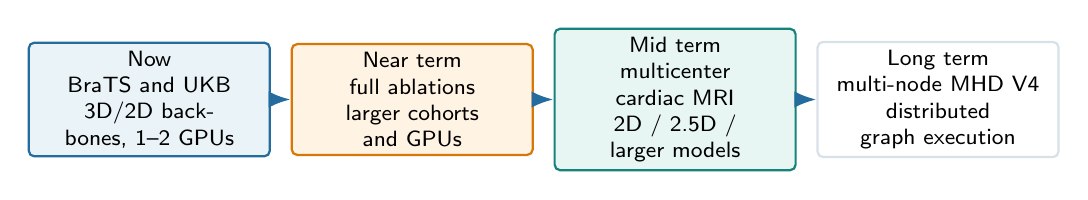
\begin{tikzpicture}[node distance=2.5mm,font=\footnotesize]
    \node[enc,text width=2.85cm] (now) {Now\\BraTS and UKB\\3D/2D backbones, 1--2 GPUs};
    \node[core,text width=2.85cm,right=of now] (near) {Near term\\full ablations\\larger cohorts and GPUs};
    \node[dec,text width=2.85cm,right=of near] (mid) {Mid term\\multicenter cardiac MRI\\2D / 2.5D / larger models};
    \node[stage,text width=2.85cm,right=of mid] (long) {Long term\\multi-node MHD V4\\distributed graph execution};
    \draw[flow] (now) -- (near);
    \draw[flow] (near) -- (mid);
    \draw[flow] (mid) -- (long);
  \end{tikzpicture}
  \vspace{5mm}
  \begin{alertblock}{Engineering constraint}
    MHD V4 represents both forward Feature Messages and backward Gradient Messages in the graph;
    the execution utilities support one- or two-GPU runs.
    Larger-memory GPUs and multi-node execution remain the path to the next scale.
  \end{alertblock}
\end{frame}

\begin{frame}{Potential TMI / MIA story: from robustness to reusable intervention}
  \begin{enumerate}
    \item \textbf{Clinical need:} multimodal imaging pipelines must remain useful under incomplete acquisition.
    \item \textbf{Technical gap:} many solutions retrain nonlinear generators or task networks for each setting.
    \item \textbf{Framework contribution:} MHD exposes reusable, ordered intervention points inside arbitrary models.
    \item \textbf{Method contribution:} LOOK estimates a compact linear residual from missing to full features.
    \item \textbf{Evidence required:} broad missingness, strong baselines, multicenter data, multiple backbones,
          efficiency, uncertainty, and matrix interpretation.
  \end{enumerate}
  \takeaway{The strongest paper is not ``one better Dice score''; it is a reusable and interpretable correction principle.}
\end{frame}

% =============================================================================
\section{Discussion}

\begin{frame}{Decisions requested from the supervisor}
  \footnotesize
  \renewcommand{\arraystretch}{0.9}
  \begin{tabularx}{\textwidth}{>{\bfseries\color{LookNavy}}p{2.7cm} Y}
    \toprule
    Decision & Concrete question \\
    \midrule
    Clinical framing & Is missing-modality segmentation the right first clinical entry point for the PhD framework? \\
    Validation priority & First complete all BraTS missing patterns, or move earlier to multicenter cardiac data? \\
    Method depth & Prioritize broad benchmark coverage or spectral/feature interpretation of $W$? \\
    Baseline budget & Which synthesis and robust-training baselines are essential for a credible TMI/MIA submission? \\
    System roadmap & When should MHD V4 multi-GPU support become a research deliverable rather than infrastructure work? \\
    \bottomrule
  \end{tabularx}
  \vspace{1.5mm}
  \begin{exampleblock}{Immediate next milestone}
    Freeze the protocol, reproduce validation, run untouched test evaluation, then expand one axis at a time.
  \end{exampleblock}
\end{frame}

\begin{frame}[plain]
  \begin{tikzpicture}[remember picture,overlay]
    \fill[LookNavy] (current page.south west) rectangle (current page.north east);
    \node[text=white,font=\bfseries\LARGE] at ([yshift=8mm]current page.center) {Thank you};
    \node[text=LookPaleBlue,font=\large,align=center] at ([yshift=-9mm]current page.center)
      {MHD V4 as the intervention framework\\LOOK as the first linear correction study};
  \end{tikzpicture}
\end{frame}

\end{document}
